\chapter{Mengenal Kecerdasan Buatan dan Scikit-Learn}
Buku umum yang digunakan adalah \cite{russell2016artificial} dan  
untuk sebelum UTS menggunakan buku \textit{Python Artificial Intelligence Projects for Beginners}\cite{eckroth2018python}.
Dengan praktek menggunakan python 3 dan editor anaconda dan library python scikit-learn.
Tujuan pembelajaran pada pertemuan pertama antara lain:
\begin{enumerate}
\item
Mengerti definisi kecerdasan buatan, sejarah kecerdasan buatan, perkembangan dan penggunaan di perusahaan
\item
Memahami cara instalasi dan pemakaian sci-kit learn
\item
Memahami cara penggunaan variabel explorer di spyder
\end{enumerate}
Tugas dengan cara dikumpulkan dengan pull request ke github dengan menggunakan latex pada repo yang dibuat oleh asisten riset.

\section{Teori}
Praktek teori penunjang yang dikerjakan :
\begin{enumerate}
\item
Buat Resume Definisi, Sejarah dan perkembangan Kecerdasan Buatan, dengan bahasa yang mudah dipahami dan dimengerti. Buatan sendiri bebas plagiat[hari ke 1](10)
\item
Buat Resume mengenai definisi supervised learning, klasifikasi, regresi dan unsupervised learning. Data set, training set dan testing set.[hari ke 1](10)
\end{enumerate}

\section{Instalasi}
Membuka https://scikit-learn.org/stable/tutorial/basic/tutorial.html. Dengan menggunakan bahasa yang mudah dimengerti dan bebas plagiat. 
Dan wajib skrinsut dari komputer sendiri.
\begin{enumerate}
\item
Instalasi library scikit dari anaconda, mencoba kompilasi dan uji coba ambil contoh kode dan lihat variabel explorer[hari ke 1](10)
\item
Mencoba Loading an example dataset, menjelaskan maksud dari tulisan tersebut dan mengartikan per baris[hari ke 1](10)
\item
Mencoba Learning and predicting, menjelaskan maksud dari tulisan tersebut dan mengartikan per baris[hari ke 2](10)
\item
mencoba Model persistence, menjelaskan maksud dari tulisan tersebut dan mengartikan per baris[hari ke 2](10)
\item 
Mencoba Conventions, menjelaskan maksud dari tulisan tersebut dan mengartikan per baris[hari ke 2](10)
\end{enumerate}


\section{Penanganan Error}
Dari percobaan yang dilakukan di atas, apabila mendapatkan error maka:

\begin{enumerate}
	\item
	skrinsut error[hari ke 2](10)
	\item
Tuliskan kode eror dan jenis errornya [hari ke 2](10)
	\item
Solusi pemecahan masalah error tersebut[hari ke 2](10)

\end{enumerate}

<<<<<<< HEAD
\section{Teori/Mhd Zulfikar Akram Nasution/1164081}
\begin{enumerate}
\item Definisi, Sejarah dan Perkembangan Kecerdasan Buatan
\begin{itemize}
\item Definisi
\par
Kecerdasan Buatan adalah kecerdasan yang ditambahkan kepada suatu sistem yang bisa diatur dalam konteks ilmiah yang berhubungan dengan pemanfaatan mesin untuk memecahkan persoalan yang rumit dengan cara yang lebih manusiawi. 
\par
\item Sejarah dan Perkembangan
\par
Sejarah dan perkembangan kecerdasan buatan terjadi pada musim panas tahun 1956 tercatat adanya seminar mengenai AI di Darmouth College. Seminar pada waktu itu dihadiri oleh sejumlah pakar komputer dan membahas potensi komputer dalam meniru kepandaian manusia. Akan tetapi perkembangan yang sering terjadi semenjak diciptakannya LISP, yaitu bahasa kecerdasan buatan yang dibuat tahun 1960 oleh John McCarthy. Istilah pada kecerdasan buatan atau Artificial Intelligence diambil dari Marvin Minsky dari MIT. Dia menulis karya ilmiah berjudul Step towards Artificial Intelligence,The Institute of radio Engineers Proceedings 49, January 1961.
\end{itemize}

\item Definisi Supervised Learning, Unsupervised Learning, Klasifikasi, Regresi, Data Set, Training Set dan Testing Set
\begin{itemize}
\item Supervised Learning dan Unsupervised Learning
\par
Supervised learning merupakan sebuah pendekatan dimana sudah terdapat data yang dilatih, dan terdapat variable yang ditargetkan sehingga tujuan dari pendekatan ini adalah mengkelompokan suatu data ke data yang sudah ada. Sedangkan unsupervised learning tidak memiliki data latih, sehingga dari data yang ada, kita mengelompokan data tersebut menjadi 2 bagian atau 3 bagian dan seterusnya.
\item Klasifikasi
\par
Klasifikasi adalah salah satu topik utama dalam data mining atau machine learning. Klasifikasi yaitu suatu pengelompokan data dimana data yang digunakan tersebut mempunyai kelas label atau target.
\item Regresi
\par
Regresi adalah Supervised learning tidak hanya mempelajari classifier, tetapi juga mempelajari fungsi yang dapat memprediksi suatu nilai numerik. Contoh, ketika diberi foto seseorang, kita ingin memprediksi umur, tinggi, dan berat orang yang ada pada foto tersebut.
\item Data Set
\par
Data set adalah cabang aplikasi dari Artificial Intelligence/Kecerdasan Buatan yang fokus pada pengembangan sebuah sistem yang mampu belajar sendiri tanpa harus berulang kali di program oleh manusia.
\item Training Set
\par
Training set yaitu jika pasangan objek, dan kelas yang menunjuk pada objek tersebut adalah suatu contoh yang telah diberi label akan menghasilkan suatu algoritma pembelajaran.
\item Testing Set
\par
Testing set digunakan untuk mengukur sejauh mana classifier berhasil melakukan klasifikasi dengan benar.
\end{itemize}
\item Instalasi Scikit-Learn dari Anaconda
\begin{itemize}
\item Pertama install Anaconda di pc masing-masing
\item Kemudian buka cmd untuk menginstall scikit-learn
\item Ketik perintah "conda install scikit-learn" dan pilih "y"
\end{itemize}
\begin{figure}[ht]
\centering
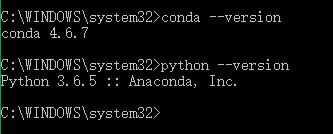
\includegraphics[scale=0.6]{figures/1.png}
\caption{Install Scikit-Learn Conda}
\label{Proses Instalasi}
\end{figure}
\begin{itemize}
\item Lalu ketik "pip install -U scikit-learn" untuk memasukkan anaconda ke python
\end{itemize}
\begin{figure}[ht]
\centering
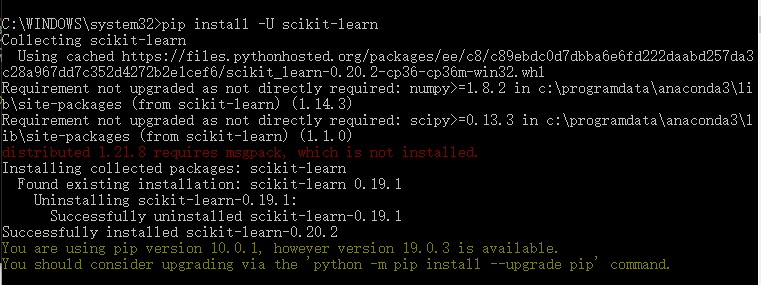
\includegraphics[scale=0.5]{figures/2.png}
\caption{Install Scikit-Learn ke Python}
\label{Gabung Conda dan Python}
\end{figure}
\begin{itemize}
\item Setelah itu, kompilasi kode di dalam python dengan ketik "python", lalu "print('Zulfikar')" maka akan menghasilkan seperti gambar berikut.
\end{itemize}
\begin{figure}[ht]
\centering
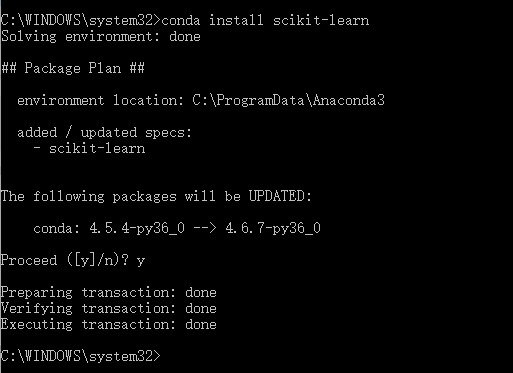
\includegraphics[scale=0.6 ]{figures/3.png}
\caption{Kompilasi Kode}
\label{Kompilasi Kode}
\end{figure}
\item Loading an Example Dataset
\begin{itemize}
\item Ketik perintah berikut "from sklearn import datasets" untuk mengimport dataset dari sklearn.
\end{itemize}
\begin{figure}[ht]
\centering
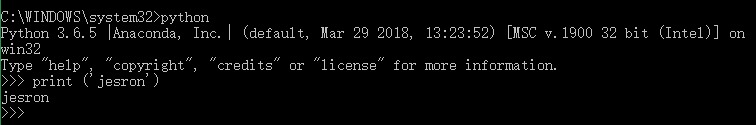
\includegraphics[scale=0.5]{figures/4.png}
\caption{Import Datasets}
\label{Import Datasets}
\end{figure}
\begin{itemize}
\item Kemudian ketik perintah berikut  untuk membuat variable iris yang berisi datasets.
\end{itemize}
\begin{figure}[ht]
\centering
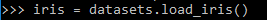
\includegraphics[scale=0.9]{figures/5.png}
\caption{Buat variable iris}
\label{Variable Iris}
\end{figure}
\begin{itemize}
\item Lalu ketik perintah berikut untuk membuat variable digits yang berisi datasets, dan juga untuk melihat isi data dari datasets seperti gambar 1.6 .
\end{itemize}
\begin{figure}[ht]
\centering
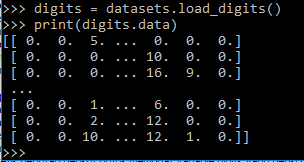
\includegraphics[scale=0.7]{figures/8.png}
\caption{Buat variable digits}
\label{Variable Digits}
\end{figure}
\end{enumerate}

\section{Jesron Marudut Hatuan/1164077}
\subsection{Teori}
\begin{enumerate}
\item Definisi, sejarah, dan perkembangan kecerdasan buatan.
\subitem Kecerdasan Buatan (Artificial Intelligence atau AI) dapat didefinisikan sebagai kecerdasan yang ditunjukkan oleh suatu entitas buatan. Sistem seperti ini biasanya dianggap komputer. Kecerdasan diciptakan lalu dimasukkan ke dalam suatu mesin atau komputer supaya dapat melakukan pekerjaan-pekerjan yang dapat dilakukan manusia.
\subitem Sebenarnya area Kecerdasan Buatan (Artificial Intelligence) atau disingkat dengan AI, dimulai dari munculanya komputer sekitar tahun 1940-an, meskipun sejarah perkembangannya dapat dilacak dari zaman Mesir kuno. Pada akhir tahun 1955, Newell dan Simon mengembangkan The Logic Theorist atau program AI terdahulu. Program ini merepresentasikan masalah sebagai model pohon, lalu penyelesaiannya dengan  memilih cabang yang akan menghasilkan kesimpulan terbenar. Program tersebut berdampak besar dan menjadi batu loncatan dalam mengembangkan bidang AI. Pada tahun 1956 John McCarthy dari  Massacuhetts Institute of Technology dianggap sebagai bapak AI, menyelenggarakan konferensi untuk menarik para ahli komputer bertemu, dengan  nama kegiatan The Dartmouth Summer Research Project On AI. Konferensi Dartmouth saat itu mempertemukan para pendiri dalam AI, dan bertugas untuk meletakkan dasar bagi masa depan  pemgembangan dan penelitian AI. John McCarthy  disaat itu mengusulkan definisi AI adalah AI merupakan cabang dari ilmu komputer yang berfokus pada pengembangan komputer agar mempunyai kemampuan dan berprilaku seperti manusia.
\item  Definisi supervised learning, klasifikasi, regresi, dan unsupervised learning. Data set, training set dan testing set. 
\subitem Supervised learning merupakan sebuah pendekatan dimana sudah terdapat data yang dilatih, dan terdapat variable yang ditargetkan sehingga tujuan dari pendekatan ini adalah mengkelompokan suatu data ke data yang sudah ada. Sedangkan unsupervised learning tidak memiliki data latih, sehingga dari data yang ada, kita mengelompokan data tersebut menjadi 2 bagian atau 3 bagian dan seterusnya.
\subitem Klasifikasi adalah salah satu topik utama dalam data mining atau machine learning. Klasifikasi yaitu suatu pengelompokan data dimana data yang digunakan tersebut mempunyai kelas label atau target.
\subitem Regresi adalah Supervised learning tidak hanya mempelajari classifier, tetapi juga mempelajari fungsi yang dapat memprediksi suatu nilai numerik. Contoh, ketika diberi foto seseorang, kita ingin memprediksi umur, tinggi, dan berat orang yang ada pada foto tersebut.
\subitem Data set adalah cabang aplikasi dari Artificial Intelligence/Kecerdasan Buatan yang fokus pada pengembangan sebuah sistem yang mampu belajar sendiri tanpa harus berulang kali di program oleh manusia.
\subitem Training set yaitu jika pasangan objek, dan kelas yang menunjuk pada objek tersebut adalah suatu contoh yang telah diberi label akan menghasilkan suatu algoritma pembelajaran.
\subitem Testing set digunakan untuk mengukur sejauh mana classifier berhasil melakukan klasifikasi dengan benar\cite{zhu2009introduction}.
\end{enumerate}


\subsection{Instalasi}
\subsubsection{Instalasi Library Scikit dari Anaconda}
\begin{enumerate}
\item Sediakan aplikasi Anaconda terlebih dahulu
\begin{figure}[ht]
\centerline{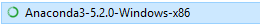
\includegraphics[width=1\textwidth]{figures/0.PNG}}
\caption{Applikasi Anaconda.}
\end{figure}
\item Setelah di install, masukkan script dibawah ini untuk melihat versi Python dan Anacondanya
\begin{figure}[ht]
\centerline{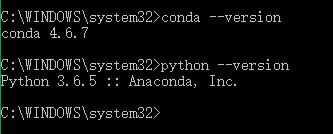
\includegraphics[width=0.75\textwidth]{figures/1.JPEG}}
\caption{Versi Anaconda.}
\end{figure}
\item  Selanjutnya masukkan perintah 'pip install -U scikit-learn'
\begin{figure}[ht]
\centerline{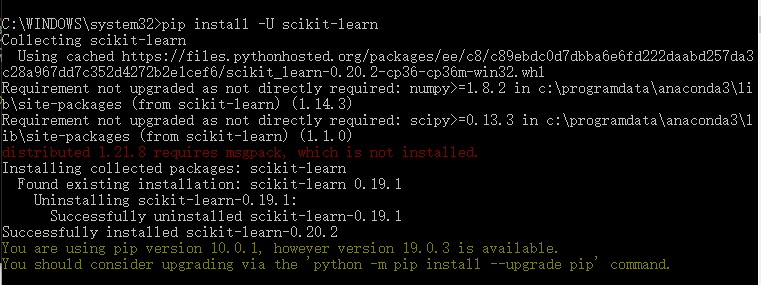
\includegraphics[width=0.75\textwidth]{figures/2.JPEG}}
\caption{Instalasi.}
\end{figure}
\item  Selanjutnya masukkan perintah 'conda install  scikit-learn'
\begin{figure}[ht]
\centerline{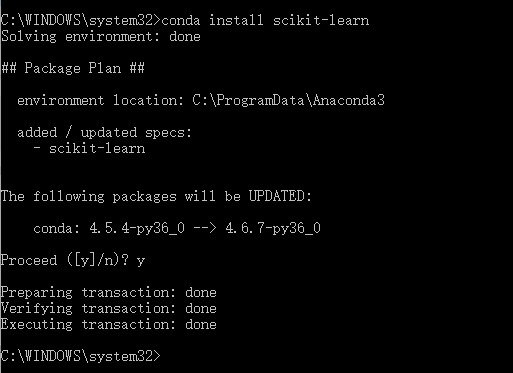
\includegraphics[width=0.75\textwidth]{figures/3.JPEG}}
\caption{Langkah installasi anaconda.}
\end{figure}
\item  Selanjutnya masukkan perintah 'python' dan 'print ('jesron')
\begin{figure}[ht]
\centerline{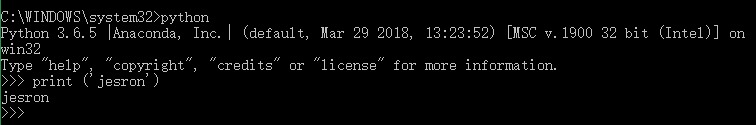
\includegraphics[width=0.5\textwidth]{figures/4.JPEG}}
\caption{Langkah terakhir.}
\end{figure}
\end{enumerate}

<<<<<<< HEAD


=======
\section{Teori/Puad Hamdani/1164084}
\begin{enumerate}
\item Definisi, Sejarah dan Perkembangan Kecerdasan Buatan
\begin{itemize}
\item Definisi
\par
Kecerdasan buatan adalah ilmu pengetahuan yang berhubungan dengan mesin untuk memecahkan persoalan rumit dengan cara yang mudah,dilakukan dengan mengikuti kecerdasan manusia dan menerapkanya di computer sebagai algoritma
\par
\item Sejarah dan Perkembangan
\par
AI (artificial Intelligence) di kenal sekitar tahun 1943 Teori tentang jaringan saraf tiruan (artificial neuron network, ANN) menyatakan bahwa setiap neuron dapat dimisalkan dalam keadaan biner, yaitu ON dan OFF. Dari setiap percobaan, setiap fungsi perhitungan dapat diselesaikan melalui jaringan neuron yang dimodelkan.
Pada tahun 1965, Lotfi Zadeh, professor teknik elektro di University of California, memublikasikan konsepnya yang disebut dengan “fuzzy sets”. Beliau menjabarkan FL dengan pernyataan matematis dan visual yang mudah dipahami. Karena kajian ini berkaitan dengan sistem kontrol, konsep tersebut banyak dikembangkan dalam konteks pemrograman komputer hingga saat ini.
\end{itemize}
\item Definisi Supervised Learning, Unsupervised Learning, Klasifikasi, Regresi, Data Set, Training Set dan Testing Set
\begin{itemize}
\item Supervised Learning 
\par
Supervised learning adalah pembelajaran yang terawasi dimana jika output yang diharapkan telah diketahui sebelumnya. Biasanya pembelajaran ini dilakukan dengan menggunakan data yang telah ada
\item Unsupervised Learning
\par
Unsupervised learning adalah pembelajaran yang tidak terawasi dimana tidak memerlukan target output. Metode ini tidak dapat ditentukan hasil seperti apa yang diharapkan selama proses pembelajaran, Nilai bobot yang disusun dalam proses range tertentu tergantung pada output yang diberikan.
\item Klasifikasi
\par
Klasifikasi adalah Proses pengelompokkan berdasarkan ciri-ciri persamaan dan perbedaan
\item Regresi
\par
Regresi adalah metode analisis statistik yang digunakan untuk melihat pengaruh antara dua atau lebih variabel
\item Data Set
\par
Data set adalah objek yang merepresentasikan data dan relasinya di memory, Strukturnya hampir mirip dengan data di data base. Data set berisi koleksi dari data table dan data relation 
\item Training Set
\par
Training set adalah bagian dataset yang kita latih untuk membuat prediksi atau algoritma ML lainnya sesuai tujuannya masing-masing. Kita memberikan petunjuk melalui algoritma agar mesin yang kita latih bisa mencari korelasinya sendiri. Walau demikian proses belajar harusnya proporsional. Layaknya seorang murid yang terlalu diforsir belajar, maka hasilnya pun tidak akan baik. Dalam istilah ML disebut dengan overfitting. Akan lebih mudah memahami konsep overfitting melalui praktek.
\item Testing Set
\end{itemize}
\par
Test set adalah bagian dataset yang kita tes untuk melihat keakuratannya, atau dengan kata lain melihat performanya.
\item Instalasi Scikit-Learn dari Anaconda
\begin{itemize}
\item Pertama install Anaconda di pc masing-masing
\item Kemudian buka cmd untuk menginstall scikit-learn
\item Ketikan "conda install scikit-learn" dan pilih "y"
\end{itemize}
\begin{figure}[ht]
\centering
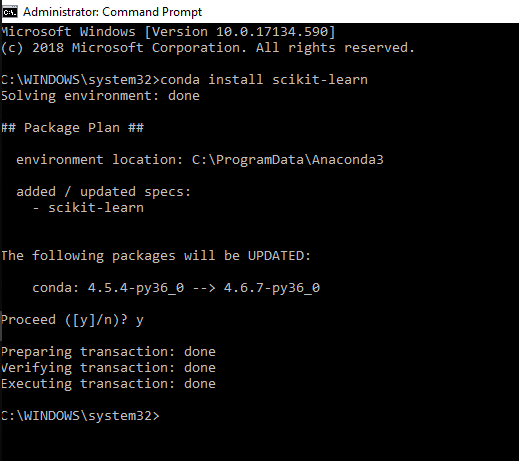
\includegraphics[scale=0.6]{figures/puad1.png}
\caption{Proses Instalasi}
\end{figure}
\begin{itemize}
\item ketik "pip install -U scikit-learn" untuk menggabungkan anaconda dan python
\end{itemize}
\begin{figure}[ht]
\centering
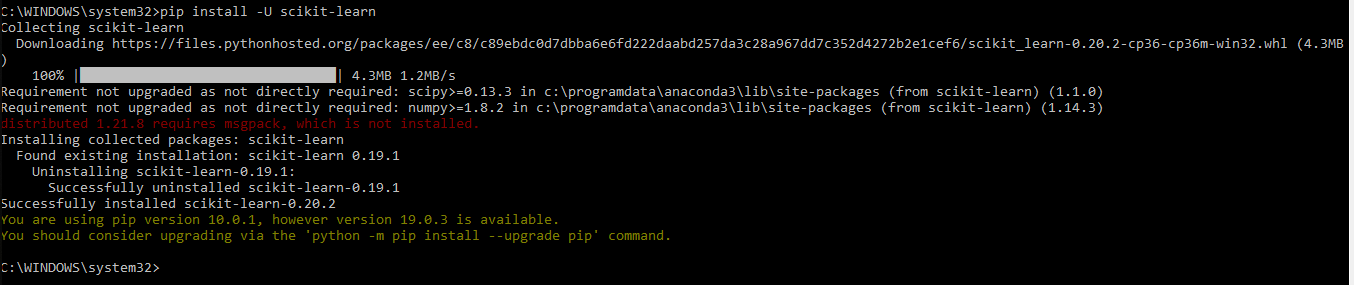
\includegraphics[scale=0.5]{figures/puad2.png}
\caption{Gabung Conda dan Python}
\end{figure}
\begin{itemize}
\item Setelah itu, kompilasi kode di dalam python dengan ketik "python", lalu "print('puad')" maka akan menghasilkan seperti gambar berikut.
\end{itemize}
\begin{figure}[ht]
\centering
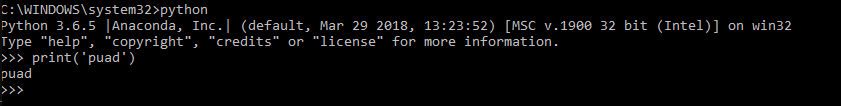
\includegraphics[scale=0.6 ]{figures/puad3.png}
\caption{Kompilasi Kode}
\end{figure}
\item Loading an Example Dataset
\begin{itemize}
\item Ketik perintah berikut "from sklearn import datasets" untuk mengimport dataset dari sklearn.
\end{itemize}
\begin{itemize}
\item ketik perintah "iris = datasets.load iris" untuk membuat variable iris yang berisi datasets.
\end{itemize}
\begin{itemize}
\item ketik perintah berikut"digits = datasets.load digits"untuk membuat variable digits yang berisi datasets, dan juga "print(digits.data) " untuk melihat isi data dari datasets seperti gambar 
\end{itemize}
\begin{figure}[ht]
\centering
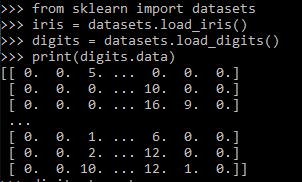
\includegraphics[scale=0.7]{figures/puad4.png}
\caption{Variable Digits}
\end{figure}
\begin{itemize}
\item kemudian  ketik "digits target"
\end{itemize}
\begin{figure}[ht]
\centering
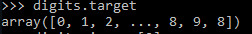
\includegraphics[scale=0.5]{figures/puad5.png}
\caption{}
\end{figure}
\begin{itemize}
\item kemudian  ketik "digits.images[0] "
\end{itemize}
\begin{figure}[ht]
\centering
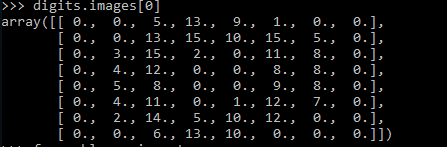
\includegraphics[scale=0.5]{figures/puad6.png}
\caption{}
\end{figure}
\begin{itemize}
\item kemudian  ketik "from sklearn import svm" dan kemudian clf = svm.SVC(gamma=0.001, C=100.) "
\item kemudian  ketik "clf.fit(digits.data[:-1], digits.target[:-1]) "
\end{itemize}
\begin{figure}[ht]
\centering
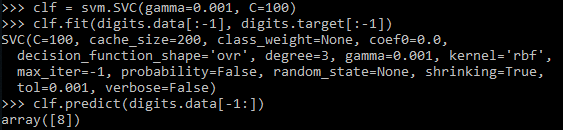
\includegraphics[scale=0.5]{figures/puad7.png}
\caption{}
\end{figure}
\begin{itemize}
\item kemudian  ketik "clf.predict(digits.data[-1:])"
\end{itemize}
\begin{figure}[ht]
\centering
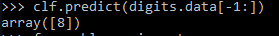
\includegraphics[scale=0.5]{figures/puad8.png}
\caption{}
\end{figure}
\begin{itemize}
\item kemudian  ketik "from sklearn import svm"
\item kemudian  ketik "from sklearn import datasets"
\item kemudian  ketik "clf = svm.SVC(gamma='scale')"
\item kemudian  ketik "iris = datasets.load(andeskore)iris()"
\item kemudian  ketik "X, y = iris.data, iris.target"
\item kemudian  ketik "clf.fit(X, y) "
\end{itemize}
\begin{figure}[ht]
\centering
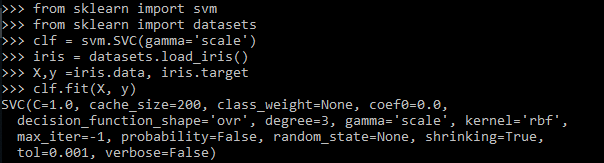
\includegraphics[scale=0.5]{figures/puad9.png}
\caption{}
\end{figure}
\begin{itemize}
\item kemudian  ketik "import pickle"
\item kemudian  ketik "s = pickle.dumps(clf)"
\item kemudian  ketik "clf2 = pickle.loads(s)"
\item kemudian  ketik "clf2.predict(X[0:1])"
\end{itemize}
\begin{figure}[ht]
\centering
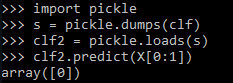
\includegraphics[scale=0.5]{figures/puad10.png}
\caption{}
\end{figure}
\begin{itemize}
\item kemudian  ketik " y[0]"
\end{itemize}
\begin{figure}[ht]
\centering
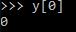
\includegraphics[scale=0.5]{figures/puad11.png}
\caption{}
\end{figure}
\begin{itemize}
\item kemudian  ketik "from joblib import dump, load"
\item kemudian  ketik "dump(clf, 'filename.joblib')"
\end{itemize}
\begin{figure}[ht]
\centering
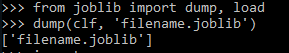
\includegraphics[scale=0.5]{figures/puad13.png}
\caption{}
\end{figure}
\begin{itemize}
\item conventions
\item ketikan "import numpy as np"
\item ketikan "from sklearn import random(andeskor)projection"
\item ketikan "rng = np.random.RandomState(0)"
\item ketikan "X = rng.rand(10, 2000)"
\item ketikan "X = np.array(X, dtype='float32')"
\item ketikan "X.dtype"
\item ketikan "transformer = random projection.GaussianRandomProjection"
\item ketikan "X new = transformer.fit transform(X)"
\item ketikan "X new.dtype"
\end{itemize}
\begin{figure}[ht]
\centering
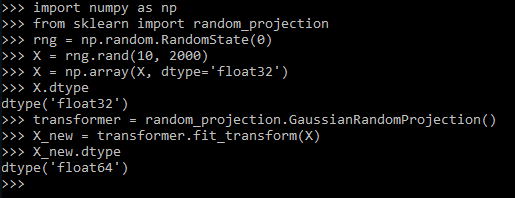
\includegraphics[scale=0.5]{figures/puad14.png}
\caption{}
\end{figure}
\item screenshoot eror
\begin{figure}[ht]
\centering
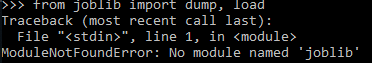
\includegraphics[scale=0.5]{figures/puad12.png}
\caption{}
\end{figure}
\item kode eror "no module named 'joblib'"
\item penanganannya instal joblib dengan mengetikan"conda instal -c anaconda joblib"
\end{enumerate}
>>>>>>> efee6eca5df5ee495d6544dd76ec774eee595c8a
=======
<<<<<<< HEAD
\section{Instalasi/Mhd Zulfikar Akram Nasution/1164081}
\begin{enumerate}
\item Menjelaskan Kode dari Learning and Predicting
\begin{itemize}
\item Pertama import file smv dari sklearn seperti pada gambar 1.12
\end{itemize}
\begin{figure}[ht]
\centering
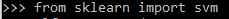
\includegraphics[scale=0.9]{figures/2_1.png}
\caption{Import file svm}
\label{Import svm}
\end{figure}
\begin{itemize}
\item Kemudian buat variabel clf seperti pada gambar 1.13
\end{itemize}
\begin{figure}[ht]
\centering
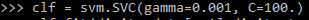
\includegraphics[scale=0.9]{figures/2_2.png}
\caption{Buat variable Classifier}
\label{Variabel clf}
\end{figure}
\begin{itemize}
\item Lalu ketik kode berikut untuk meliat array baru dari syntax python [:-1] sepert padai gambar 1.14
\end{itemize}
\begin{figure}[ht]
\centering
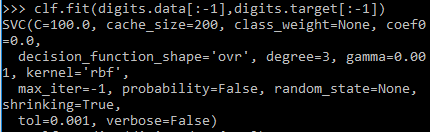
\includegraphics[scale=0.7]{figures/2_3.png}
\caption{Lihat array baru dengan syntac Python}
\label{Syntax python}
\end{figure}
\begin{itemize}
\item Selanjutnya ketikkan kode berikut untuk melihat penggolongan array seperti pada gambar 1.15
\end{itemize}
\begin{figure}[ht]
\centering
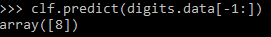
\includegraphics[scale=0.7]{figures/2_4.png}
\caption{Lihat classifier array}
\label{Classifier Array}
\end{figure}
\item Model Persistence
\begin{itemize}
\item Pertama Import dulu file dari sklearn
\end{itemize}
\begin{figure}[ht]
\centering
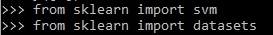
\includegraphics[scale=0.7]{figures/2_5.png}
\caption{Import file}
\end{figure}
\begin{itemize}
\item Kemudian buat variable classifier dengan gamma=scale
\end{itemize}
\begin{figure}[ht]
\centering
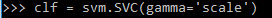
\includegraphics[scale=0.9]{figures/2_6.png}
\caption{Variable classifier}
\end{figure}
\begin{itemize}
\item Lalu buat variable iris dan (X,y)
\end{itemize}
\begin{figure}[ht]
\centering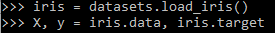
\includegraphics[scale=0.9]{figures/2_7.png}
\caption{Variable iris}
\end{figure}
\begin{itemize}
\item Selanjutnya kita akan melihat penyesuaian classifier
\end{itemize}
\begin{figure}[ht]
\centering
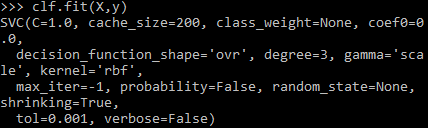
\includegraphics[scale=0.7]{figures/2_8.png}
\caption{Penyesuaian Classifier}
\end{figure}
\begin{itemize}
\item Kemudian import pickle untuk melihat hasil array dan hasil y
\end{itemize}
\begin{figure}[ht]
\centering
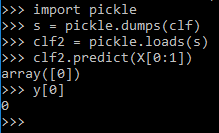
\includegraphics[scale=0.7]{figures/2_9.png}
\caption{Import Pickle}
\end{figure}
\item Conventions
\begin{itemize}
\item Pertama import numpy menjadi np serta import random projection
\end{itemize}
\begin{figure}[ht]
\centering
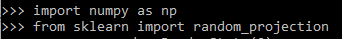
\includegraphics[scale=0.7]{figures/2_10.png}
\caption{Import numpy}
\end{figure}
\begin{itemize}
\item Kemudian buat variable rng dengan type random
\end{itemize}
\begin{figure}[ht]
\centering
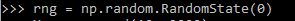
\includegraphics[scale=0.7]{figures/2_11.png}
\caption{Variable rng}
\end{figure}
\begin{itemize}
\item Lalu buat variable X, dan lihat hasil rng random yang keluar
\end{itemize}
\begin{figure}[ht]
\centering
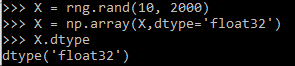
\includegraphics[scale=0.9]{figures/2_12.png}
\caption{Variable X dan hasil random}
\end{figure}
\begin{itemize}
\item Setelah itu buat variable transformer dengan type random
\end{itemize}
\begin{figure}[ht]
\centering
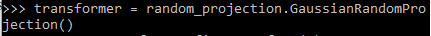
\includegraphics[scale=0.9]{figures/2_13.png}
\caption{Variable transformer random}
\end{figure}
\begin{itemize}
\item Berikutnya itu buat variable X new dengan type yang ada pada tranformer
\end{itemize}
\begin{figure}[ht]
\centering
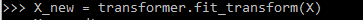
\includegraphics[scale=0.9]{figures/2_14.png}
\caption{Variable X new type pada transformer}
\end{figure}
\begin{itemize}
\item Kemudian lihat hasil dari X new
\end{itemize}
\begin{figure}[ht]
\centering
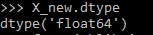
\includegraphics[scale=0.9]{figures/2_15.png}
\caption{Hasil dari X new type pada transformer}
\end{figure}
\item Screenshoot Error pada gambar 1.27
\begin{figure}[ht]
\centering
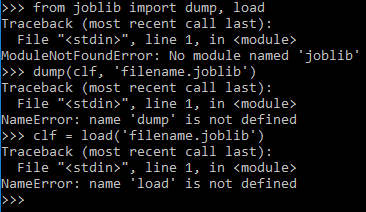
\includegraphics[scale=0.7]{figures/2_16.png}
\caption{Screenshoot Error}
\end{figure}
\item Kode yang error yaitu "joblib" karena belum ada library nya seperti pada gambar 1.28
\item Solusi dari masalah yang error seperti pada gambar 1.29
\begin{figure}[ht]
\centering
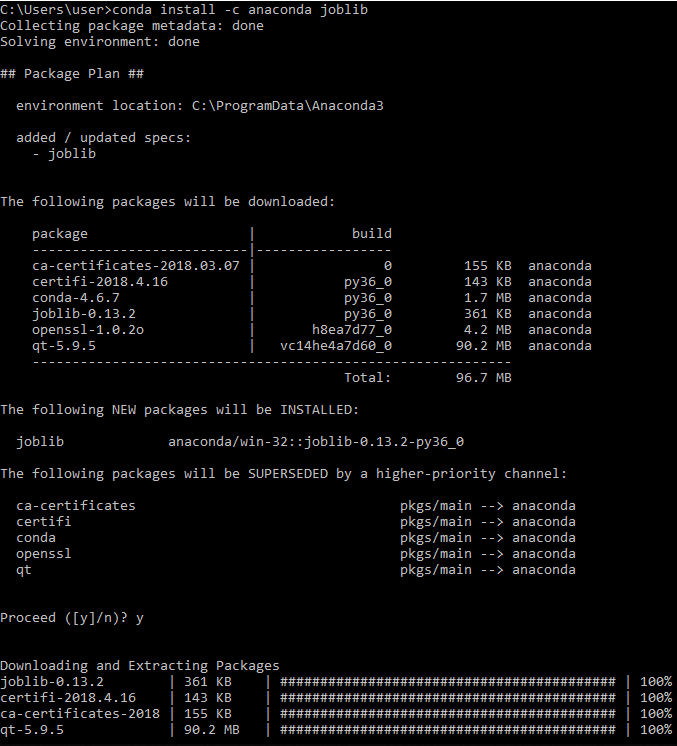
\includegraphics[scale=0.3]{figures/2_17.png}
\caption{Install Joblib}
\end{figure}
\begin{figure}[ht]
\centering
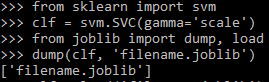
\includegraphics[scale=0.7]{figures/2_18.png}
\caption{Solusi Error}
\end{figure}


\end{enumerate}
=======
\subsection{Installasi}
\subsubsection{Loading an Example Datasets}
\begin{enumerate}
\item Loading an Example Dataset
\begin{itemize}
\item Ketik perintah berikut "from sklearn import datasets" untuk mengimport dataset dari file sklearn tadi.
\end{itemize}
\begin{figure}[ht]
\centering
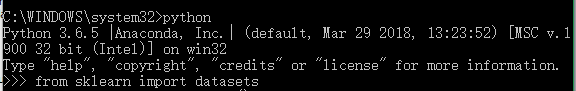
\includegraphics[scale=0.5]{figures/satu.png}
\caption{Perintah sklearn import datasets}
\label{Import Datasets}
\end{figure}
\begin{itemize}
\item Selanjutnya ketik perintah berikut ini untuk membuat variable iris yang berisi datasets.
\end{itemize}
\begin{figure}[ht]
\centering
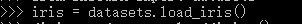
\includegraphics[scale=0.9]{figures/dua.png}
\caption{Perintah Variabel Iris}
\label{Variable Iris}
\end{figure}
\begin{itemize}
\item Masukkan perintah ini untuk membuat variable digits yang berisi datasets, dapat juga untuk melihat isi data dari datasets tadi.
\end{itemize}
\begin{figure}[ht]
\centering
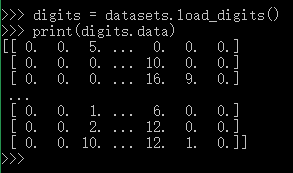
\includegraphics[scale=0.9]{figures/tiga.png}
\caption{Perintah Variabel Digits}
\label{Variable Digits}
\end{figure}
\end{enumerate}


\section{Learning and Predicting}
\begin{itemize}
\item from sklearn import svm ( pada baris berikut ini merupakan sebuah perintah untuk mengimport class svm dari package sklearn).
\item clf = svm.SVC (gamma=0.001, C=100.) (pada baris kedua ini clf sebagai estimator atau parameter, svm.SVC menjadi sebuah class, dan gamma sebagai parameter untuk menetapkan nilai secara manual)
\item clf.fit(digits.data[:-1], digits.target[:-1]) (pada baris ketiga ini clf sebagai estimator atau parameter, fit sebagai metode, digits.data sebagai item, [:-1] sebagai syntax pythonnya dan menampilkan outputannya)
\item clf.predict(digits.data[-1:])
\end{itemize}
\subsubsection{Model Presistence}
\begin{itemize}
\item from sklearn import svm
\item from sklearn import datasets
\item clf = svm.SVC(gamma='scale')
\item iris = datasets.load\_iris()
\item X, y = iris.data, iris.target
\item clf.fit(X, y)hasil
\item import pickle
\item s = pickle.dumps(clf)
\item clf2 = pickle.loads(s)
\item clf2.predict(X[0:1])hasil
\item y[0]hasil
\item from joblib import dump, load eror
\item dump(clf, 'filename.joblib')eror
\item clf = load('filename.joblib')eror
\end{itemize}
\subsubsection{Conventions}
\begin{enumerate}
\item Type Casting
\begin{itemize}
\item from sklearn import svm
\item from sklearn import random\_projection
\item rng = np.random.RandomState(0)
\item X = rng.rand(10, 2000)
\item X = np.array(X, dtype='float32')
\item X.dtype hasil
\item transformer = random\_projection.GaussianRandomProjection()
\item X\_new = transformer.fit\_transform(X)
\item X\_new.dtype hasil
\item from sklearn import datasets
\item from sklearn.svm import SVC
\item iris = datasets.load\_iris()
\item clf = SVC(gamma='scale')
\item clf.fit(iris.data, iris.target)hasil
\item list(clf.predict(iris.data[:3])) hasil
\item clf.fit(iris.data, iris.target\_names[iris.target]) hasil
\item list(clf.predict(iris.data[:3])) hasil
\end{itemize}
\item Refitting and Updating Parameters
\begin{itemize}
\item import numpy as np
\item from sklearn.svm import SVC
\item rng = np.random.RandomState(0)
\item X = rng.rand(100, 10)
\item y = rng.binomial(1, 0.5, 100)
\item X\_test = rng.rand(5, 10)
\item clf = SVC()
\item clf.set\_params(kernel='linear').fit(X, y) hasil
\item clf.predict(X\_test) hasil
\item clf.set\_params(kernel='rbf', gamma='scale').fit(X, y) hasil
\item clf.predict(X\_test) hasil
\end{itemize}
\item Multiclass vs. Multilabel Fitting
\begin{itemize}
\item from sklearn.svm import SVC
\item from sklearn.multiclass import OneVsRestClassifier
\item from sklearn.preprocessing import LabelBinarizer
\item X = [[1, 2], [2, 4], [4, 5], [3, 2], [3, 1]]
\item y = [0, 0, 1, 1, 2]
\item classif = OneVsRestClassifier(estimator=SVC(gamma='scale',random\_state=0))
\item classif.fit(X, y).predict(X) hasil
\item y = LabelBinarizer().fit\_transform(y)
\item classif.fit(X, y).predict(X) hasil
\item from sklearn.preprocessing import MultiLabelBinarizer
\item y = [[0, 1], [0, 2], [1, 3], [0, 2, 3], [2, 4]]
\item y = MultiLabelBinarizer().fit\_transform(y)
\item classif.fit(X, y).predict(X) hasil
\end{itemize}
\end{enumerate}

\section{Penanganan Error}
\begin{enumerate}
\item
Dibawah ini merupakan error yang ditemukan pada saat melakukan percobaan import.
\begin{figure}
\begin{center}
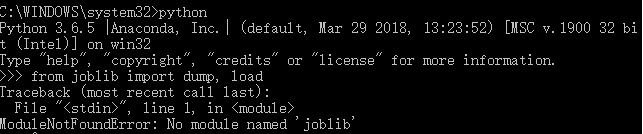
\includegraphics[scale=0.75]{figures/Error1.png}
\caption{Error Import}
\end{center}
\end{figure}
\item
Pada gambar diatas, terjadi error ketika sedang mengimport modul yang telah ditetapkan.
\item
Solusinya dapat dilakukan dengan berikut ini :\\
Error tadi terjadi akibat Library Joblib pada PC belum terinstall. Oleh sebab itu, install terlebih dahulu.
\item
Dengan membuka CMD (Admin), kemudian masukkan perintah "pip install joblib" dan tunggu sampai installasi berhasil seperti gambar berikut.
\begin{figure}
\begin{center}
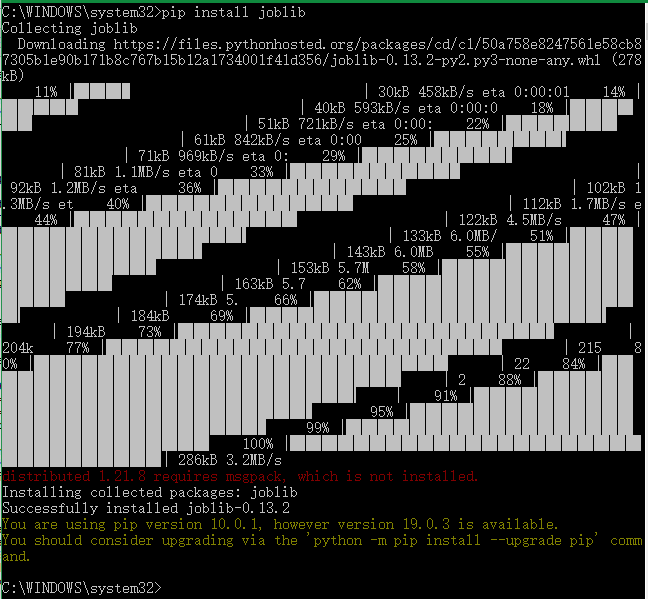
\includegraphics[scale=0.5]{figures/install2.png}
\caption{Install Library Joblib}
\end{center}
\end{figure}
\item
Ketika sudah terinstall, maka bisa dilakukan lagi import library joblib, dan hasilnya akan tampil seperti dibawah ini
\begin{figure}
\begin{center}
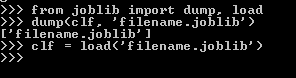
\includegraphics[scale=1]{figures/hasil3.png}
\caption{Berhasil Import Library Joblib}
\end{center}
\end{figure}
\end{enumerate}




>>>>>>> 
>>>>>>> f594df5d4cf2e0a7297e57a9c544d6f3fac837ab
>>>>>>> 2951ffb45da2a049bd0331edf27d34ed0e23f9f5
